\chapter{The role of science communication}
This chapters presents a concise overview of the importance of science communication in modern society. Section \ref{The_knowledge_era} outlines the characteristics of the knowledge era. Section \ref{Challenges_in_the_knowledge_era} focuses on the related economical and societal challenges. Section \ref{The_scientific_citizenship} highlights the need for scientific citizenship in the knowledge era. Section \ref{The_scientific_citizenship} presents science communication as a requirement for scientific citizenship. 

\section{The knowledge era} \label{The_knowledge_era}
Three economical eras have been identified in the history of human civilisation \cite{Aasi1}. The first one was the agricultural era. This is believed to have started between 10000 and 8000 B.C. in different regions in the world. The second one is the industrial era. It began in England in the 18th century as a result of the industrial revolution. The third one is the knowledge era, and it is the age into which human civilization is currently entering. 

The three eras are based on different primary production resources. The agricultural age was founded on the work of people and animals. The ultimate source of richness and development in the industrial era was the work of people and machines. Finally, the current era is not based on the capacity to produce and accumulate tangible goods, but rather on the ability to store, generate and apply new knowledge.

The information on which the current era is based is mainly scientific. In the past centuries, the impact of science on humanity has been growing without interruption. Nowadays, the outcomes of scientific activities permeate our society and heavily shape our life style. Examples range from telecommunications to medicine, or from artificial intelligence to the development of new materials.

The reason for the increasing impact of science is the peculiar nature of scientific knowledge as a resource. Just like any other resource, it is important for its capacity to provide solutions to problems. However, contrarily to resources such as water, food or oil, scientific knowledge is potentially unlimited, as it is capable of generating itself (knowledge leads to new knowledge). Moreover, the same knowledge can be used simultaneously by multiple entities. Hence, scientific knowledge is intrinsically a non-exclusive good.

For its characteristics as a resource, scientific knowledge has revolutionised the world economy. The current science-driven change of the global market has introduced countless positive innovations. However, it has also led to dramatic societal changes.   

\section{Challenges in the knowledge era} \label{Challenges_in_the_knowledge_era}
The relationship between scientific research and society has changed significantly after the second world war. From the second half of the 20th century, several countries have started using science and its generation of new knowledge and technology as a source of economical growth. This process has progressively become more intense over the last decades. Nowadays, nations invest significant fractions of their gross domestic product in research and development. Examples are the European Union, the United States, and Asiatic countries such as China and South Korea, see figure \ref{GD_investment}.    

\begin{figure}[!t] 
 \begin{center}
 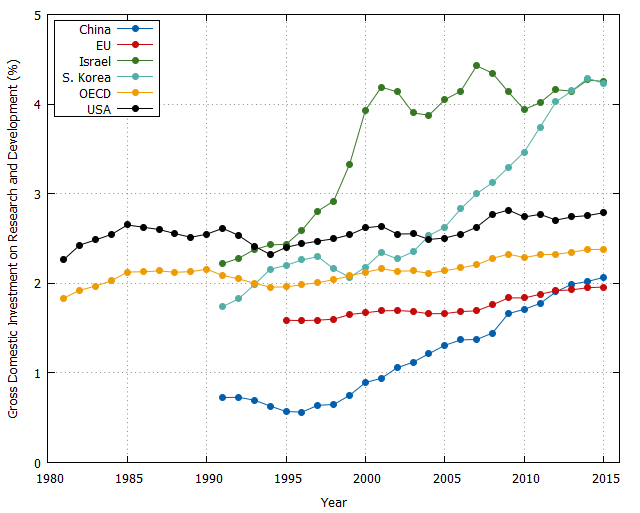
\includegraphics[scale=0.3]{Images/GD_investment.png}
 \caption{Gross domestic percentage invested in science and development over the past years by some of the world's leading economies. The image is based on data of the ...}
 \label{GD_investment}
 \end{center}
\end{figure}

The capacity of scientific knowledge to generate richness has attracted a growing number of private investors. As a result, in many countries private investment on scientific research is larger than public funds. One example are the United States, where the former is currently twice as large as the latter. 

\begin{figure}[!t] 
 \begin{center}
 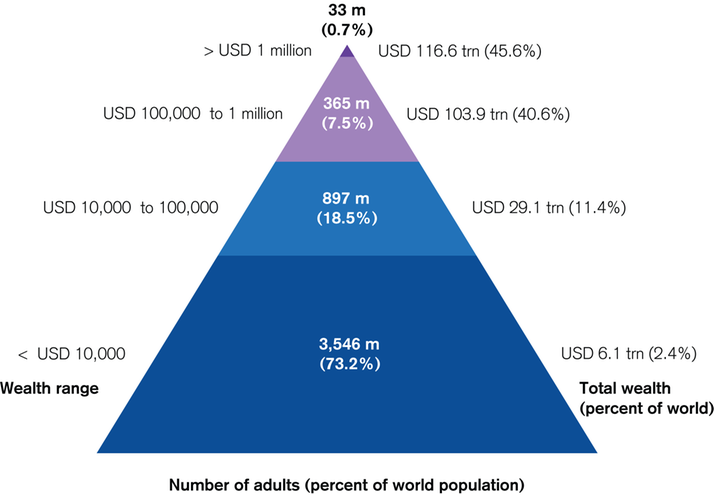
\includegraphics[scale=0.3]{Images/Global_wealth_pyramid.png}
 \caption{Distribution of the global wealth among the world's population. Original image in ...}
 \label{Global_wealth_pyramid}
 \end{center}
\end{figure}

The leading role of private investors is based on a reinterpretation of knowledge as a resource. To pursue personal profit, investors are typically non interested in sharing the knowledge they develop or they way they use it to create goods. This approach limits the possibility to generate new knowledge from the results of others. Moreover, people with limited buying power cannot afford specific classes of products and benefit from the knowledge behind them. One example are patented expensive medicines. In such a scenario, knowledge as a resource partially looses the intrinsic characteristics mentioned in Section \ref{The_knowledge_era} of being unlimited and non exclusive. 

\begin{figure}[!t] 
 \begin{center}
 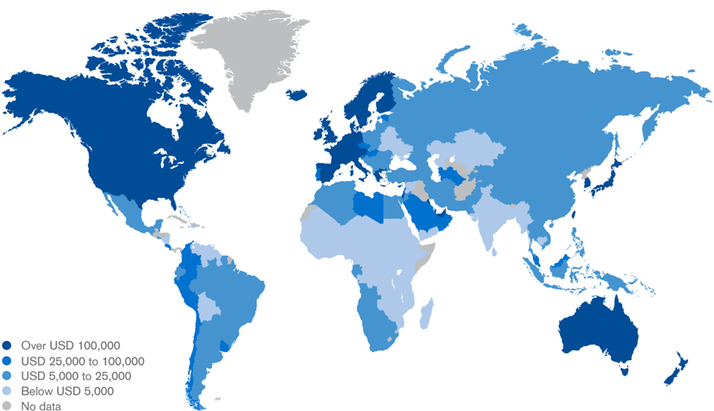
\includegraphics[scale=0.3]{Images/World_wealth_levels.png}
 \caption{Comparison among nations of the current annual wealth per adult. Original image in ...}
 \label{World_wealth_levels}
 \end{center}
\end{figure}

The current knowledge-driven development of the global economy has two important consequences. Firstly, humanity is richer than ever before. Secondly, the progressive concentration of the generated richness in the hands of few individuals is causing societal inequality, see figures \ref{Global_wealth_pyramid} and \ref{World_wealth_levels}. 

The increasing inequality is an obstacle for the creation of a democratic society. The scenario humanity is facing can change if knowledge will not be used as a mere instrument of power, but rather as a common good everyone should benefit from. This paradigm shift can be achieved through the acquisition of the scientific citizenship.

\section{The scientific citizenship} \label{The_scientific_citizenship}
The potential of scientific knowledge to be a pillar of democratic societies was first recognised by English philosopher Francis Bacon in the 17th century. He proposed that science and technology should not bring advantages to a limited number of societal groups or nations, but rather to the whole humankind. This vision is efficaciously outlined in his utopian novel \textit{New Atlantis}.

Bacon's ideas are extremely topical. As mentioned in section \ref{Challenges_in_the_knowledge_era}, the equal access to goods generated by scientific research is fundamental to prevent societal divisions and exclusions.

A second ingredient for the creation of a democratic society is the people's awareness of the scientific process, as well as of its goals, outcomes and limits. In fact, democratic societies are founded on the engagement of citizens when decisions impacting the community must be taken. Because of science permeating role in today's society, science-related issues are no exception. Examples are topics such as mandatory vaccination, euthanasia, abortion, animal experimentation, alternative medicine, nuclear energy, recycling and, in general, the public investments on research assigned by policy makers. Hence, a better understanding of science is a key factor to ensure effective participatory processes.    

The population's engagement in decision-making processes is only fruitful if scientific innovations are neither passively accepted nor irrationally feared. To this aim, people must be given the ability to intervene in an informed, rational and critical way. This scenario is only possible if individuals are formed and trained in an adequate cultural context. In other words, if people acquire the so-called scientific citizenship.

How to best prepare individuals to become scientific citizens is still debated. Nevertheless, a key ingredient has been identified in the need to bring scientists and citizens closer to each other. It is widely accepted that the construction of a democratic knowledge era depends crucially on the continuous dialogue and information and knowledge exchange between these two communities. A paradigm which motivates the growing importance of science communication.

\section{Science communication and modern society}    
Science relies heavily on communication. To be useful, research results must be communicated to the rest of the scientific community. This has become even more crucial in the era of Big Science. Modern physics offers illustrative examples in this direction. Large-scale experiments such as the LHC particle accelerator at CERN in Switzerland or the LIGO-Virgo gravitational-wave observatories in the USA and Italy are built and maintained by international collaborations of thousands of scientists from tens of different countries. These titanic efforts can only be successful if supported by effective internal communication.  

The relationship between science and communication has evolved with the transition to the knowledge era. Nowadays, science communication can no longer happen exclusively within the scientific community. As outlined in Section \ref{The_scientific_citizenship}, the construction of a democratic society requires the engagement of disparate societal groups in the decision-making processes related to scientific questions. Examples are scientists, policy makers, private investors, non-governmental organizations, citizens etc. Hence, when discussing with each other, these groups make use of science communication.

The aforementioned societal groups have different cultural background and objectives. Thus, they adopt different languages when talking about scientific issues. Moreover, to be effective, each group must tune its science communication on the targeted audience, with the optimal choice depending on both the content and considered communication channel. As a consequence, numerous different kinds of science communication can be identified.   

The present thesis focuses on science communication aiming to inform citizens on a non-technical level of current investigation lines. This is the oldest type of science communication not confined within the scientific community. The first example in this direction was the \textit{De Rerum Natura} by Roman poet Lucretius in the first century BC. Another historically very important book was Galileo Galiei's \textit{Sidereus Nuncius} in the XVII century. His work rapidly spread all over the world short after publication and revolutionised humanity's self-perception by propagating the author's innovative astronomical discoveries.

More specifically, this thesis focuses on a specific class of EU-funded research project and on their use of the web 2.0 social media to communicate results and objectives. As outlined in the next chapters, the ultimate goal is to investigate whether European scientists are properly exploiting today's most effective communication channels to inform citizens of two of the future's most important scientific challenges: the development of quantum technologies and supercomputers.

\section{Chapter summary} 
In this chapter, the following items have been discussed:

\begin{enumerate}
 \item Human society is currently entering the so-called knowledge era. This age is characterised by the fact that scientific knowledge has become one of the most important sources of wealth. 
 \item The knowledge era offers unprecedented opportunities to improve people's life quality. However, it also presents new challenges. In particular, the unequal access to scientific knowledge and technology may prevent the realisation of democratic systems.
 \item The construction of a democratic society in the knowledge era depends on the engagement of citizens and stakeholders in the debate on the impact of scientific issues on their lives. This can be achieved by training people to discuss scientific questions in a constructive and critic way, i.e., if individuals acquire the so-called scientific citizenship.
 \item One key factor to help people acquire the scientific citizenship is science communication. There exist disparate kinds of science communication, depending on the interacting societal groups. The present thesis focuses on science communication adopted to inform citizens via social media of recent developments in European research projects.     
\end{enumerate}